\documentclass{article}
\usepackage[utf8]{inputenc}
\usepackage{tikz}
\title{lab6_dop}
\author{Арсений Векшин}
\date{November 2022}

\begin{document}

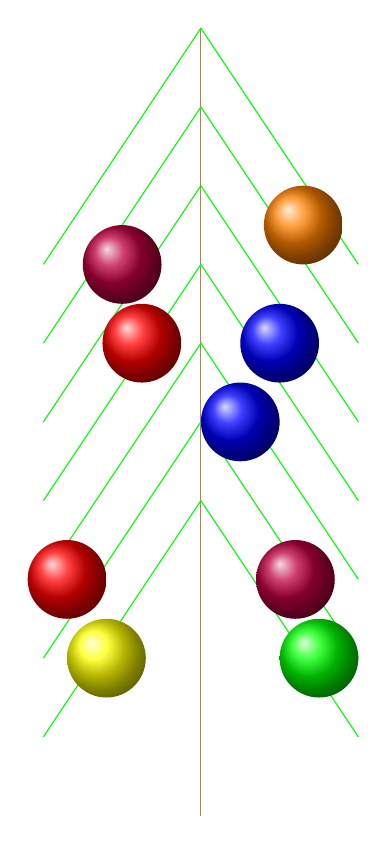
\begin{tikzpicture}
\draw[color=brown] (0,0) -- (0,10);
\draw[color=green] (-2,7) -- (0,10) -- (2,7);
\draw[color=green] (-2,6) -- (0,9) -- (2,6);
\draw[color=green] (-2,5) -- (0,8) -- (2,5);
\draw[color=green] (-2,4) -- (0,7) -- (2,4);
\draw[color=green] (-2,3) -- (0,6) -- (2,3);
\draw[color=green] (-2,2) -- (0,5) -- (2,2);
\draw[color=green] (-2,1) -- (0,4) -- (2,1);

\shade[ball color=green]    (1.5,2) circle(0.5);
\shade[ball color=red]      (-1.7,3) circle(0.5);
\shade[ball color=blue] 	(1,6) circle(0.5);
\shade[ball color=purple] 	(-1,7) circle(0.5);
\shade[ball color=red] 		(-0.75,6) circle(0.5);
\shade[ball color=yellow] 	(-1.2,2) circle(0.5);
\shade[ball color=orange] 	(1.3,7.5) circle(0.5);
\shade[ball color=blue] 	(0.5,5) circle(0.5);
\shade[ball color=purple] 	(1.2,3) circle(0.5);

\end{tikzpicture}


\end{document}
